\title{Computer Architecture - CS 301} % You may change the title if you want.

\author{Rishit Saiya - 180010027, Assignment - 10}

\date{\today}

\documentclass[12pt]{article}
\usepackage{fullpage}
\usepackage{enumitem}
\usepackage{amsmath,mathtools}
\usepackage{amssymb}
\usepackage[super]{nth}
\usepackage{textcomp}
\usepackage{hyperref}
\hypersetup{
    colorlinks=true,
    linkcolor=blue,
    filecolor=magenta,      
    urlcolor=cyan,
}
\begin{document}
\maketitle

%----------------------------------------------------------------
We have an inclusion Cache Hierarchy as given in Figure 1. We revolve around this to explain Write-Back and Write policies. So, if any address exists in L1 cache, the same address will also be present in L2 cache. However block in L1 cache can have newer data. So, this is the main idea around which we will build upon the ways to write in caches. So, by basic idea of cache, we follow the fundamental logic as follows:
\begin{verbatim}
    bool compare = Compare data ((Find in L2) || (Find in L1));
    if(compare){
       Fetch directly;
    }
    else {
       Fetch from Memory;
       Write in a block in cache;
    }
\end{verbatim}

The basic explanation being that if the block of memory exists in any of the levels of internal cache hierarchy, then fetch it directly or else fetch it from memory and include in a block in cache while fetching for immediate use in further instructions. Below we shall discuss about techniques which will write in cache in the process of fetching data from memory :- Write-Back \& Write Through Techniques.


\begin{figure}
    \centering
    % 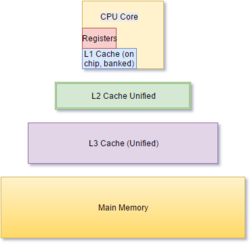
\includegraphics[width=3cm,height=3cm]{Assignment-10/Cache_Hierarchy_Updated.png}
    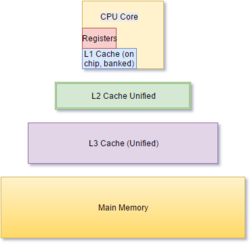
\includegraphics{Assignment-10/Cache_Hierarchy_Updated.png}
    \caption{Inclusive Cache Hierarchy}
\end{figure}


\section{}
\textbf{\textit{Write-back:}} \\
As directly mentioned in the video lecture, Write-Back process in simple terms is described as whenever we write to cache, we do not write to the lower level. If we write, we set the modified bit to 1. Now let's try to understand it on internal level.

First of all, we need to understand about the modified/dirty bit. It is actually defined as a bit that is associated with a block of computer memory and indicates whether or not the corresponding block of memory has been modified. In simple terms, it is an extra bit attached to the tag and it is set to 0 and 1 accordingly.
Figure 2 shows the representation of Modified Bit in the One Cache Line.

\begin{figure}
    \centering
    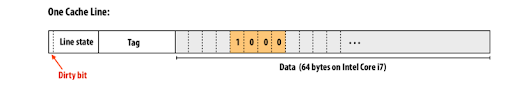
\includegraphics{Assignment-10/modified_bit.png}
    \caption{Modified Bit}
\end{figure}

A small advantage of Write-Back over Write-Through is that for every data call from Cache, we don't have go till L2 and hence we save power, computations and traffic to L2. It is clearly depicted in Figure 3. Instead in Write-Back is populates in L1 and sets the Modified Bit to 1. \\

\begin{figure}
    \centering
    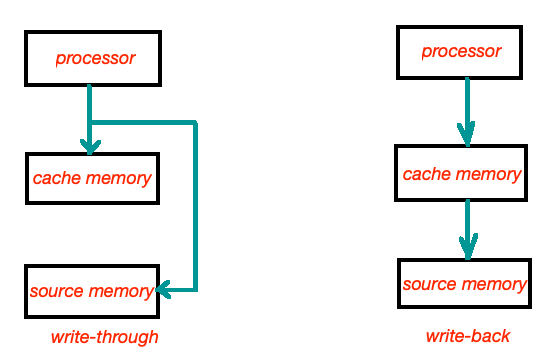
\includegraphics[scale=0.5]{Assignment-10/data-cache.png}
    \caption{Difference in workflow of Write-Back and Write-Through}
\end{figure}

\textbf{\textit{Write-Through:}} \\
As directly mentioned in the video lecture, Write-Through process in simple terms is described as whenever we write to cache, we also write to lower level. Now let's try to understand it on internal level.

By using the Property of Inclusion, if we write any block in L1, by principle, it will get propagated in L2 consecutively too. In general, there is no need of modified bit in this case. So, this gives us the privilege to throw data a certain block from the cache as per convenience. 

A small advantage of Write-Through over Write-Back is the ease of eviction of data process. In Write-Back, we have to check the following logic for eviction of data from cache:
\begin{verbatim}
    int modified_bit;
    // After Cache Process ...
    if(modified_bit){
       Write the block in lower level;
       Dump;
    }
    else {
       Dump;
    }
\end{verbatim}

So, the above process takes place in Write-Back and on the other hand in Write-Through, the eviction process is quite direct.
%----------------------------------------------------------------

\section{}
By looking over the past instructions and based upon the use of the busy lines and probability of using lines where the usage will be minimum is the line to be evicted. To get a systematic hold of such a process Least Recently Used (LRU) Technique helps us to get such lines' eviction easier. In this method, we replace an entry in the set by a new entry. \\

In the video lecture, there is a mention of FIFO (First in First Out) Replacement policy where the one block that is first inserted is the one to be taken out first. But if the case is such that $1^{st}$ inserted block usage frequency is high, then our process of eviction becomes completely fatal. So, this is clearly not that effective technique. \\

The video lecture also touches upon the fact of using Random Replacement Policy, where random blocks are evicted. But even this is useless as the most frequently used block might be evicted and not so frequently used block might stay in Cache. So, this is also not an effective technique. \\

The whole purpose of technique of LRU is to gain easier access to frequently used data blocks in compliance with Temporal Locality Rules. But as we saw above, Random Replacement Policy \& FIFO Replacement Policy potentially can violate the rules of temporal locality whereas LRU doesn't. \\

With the motive, I mentioned in the 1st paragraph where LRU adapts such that it replaces the block that has been accessed the least in recent past and the probability of that it will be used in near future is less. So, LRU is better Replacement Technique with above considerations. \\

But in the lecture video it is mentioned that LRU is difficult to implement because of various factors like bulky timestamps and with limited resources from hardware, the implementation is real challenge. So, to serve similar purpose, we come up with Pseudo-LRU instead of hardcore implementation of LRU. \\

In this implementation, we mark the Most Recently Used (MRU) Elements. It is done in following logic:
\begin{verbatim}
    
\end{verbatim}
\begin{itemize}
    \item First we associate a 3 bit counter with every way.
    \item Whenever we access a line, we increment the counter.
    \item We stop incrementing beyond 7.
    \item We periodically decrement all the counters in a set by 1.
    \item Set the counter to 7 for a newly fetched block.
    \item For replacement, choose the block with the smallest counter.
\end{itemize}

We set the counter to 7 for a newly fetched block as it is most likely to be accessed again in near future.
%----------------------------------------------------------------
\end{document}